\documentclass[11pt]{article}
\usepackage[paper=letterpaper, left=1in, right=1in, top=1in, bottom=1in]
           {geometry}
\usepackage[parfill]{parskip}
\usepackage{amsmath}
\usepackage[siunitx]{circuitikz}
\usepackage{color}
\usepackage{graphicx}

\newcommand{\problem}[1]{\textbf{Problem #1 ---} }
\newcommand{\answer}{{\color{red}\textit{Answer: }}}
\newcommand{\amp}{\ampere}

\begin{document}
\thispagestyle{empty}

\begin{center}
{\large CS330 Architecture and Organization}\\
Assignment Appendix B
\end{center}

\begin{flushright}
Your Name Here %%% <- FIXME
\end{flushright}

\problem{B.2}(5 points) In addition to the basic laws we discussed in this section, there are two important theorems, called DeMorgan's theorems:
\[ \overline{A+B} = \overline{A}\cdot\overline{B} \text{ and } \overline{A\cdot B}=\overline{A}+\overline{B} \]
Prove that the two equations for $E$ in the example starting on page B-7 are equivalent by using DeMorgan's theorems and the axioms shown on page B-7. (Section B.2)

\answer
Answer here.

\problem{B.4}(6 points) One logic function that is used for a variety of purposes (including within adders and to compute parity) is \textit{exclusive OR}.  The output of a two-input exclusive OR function is true only if exactly one of the inputs is true.  Show the truth table for an exclusive OR function and implement this function using AND gates, OR gates, and inverters. (Section B.4)

\answer
You may draw this solution and upload an image, or include it here:
%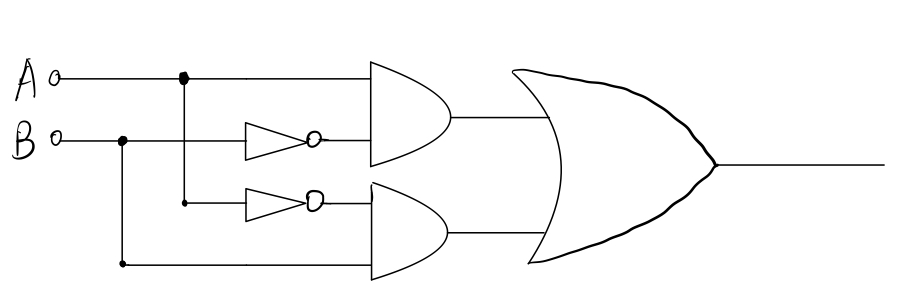
\includegraphics{answerB4.png}

\problem{B.6}(5 points) Prove that the NAND gate is universal by showing how to build the AND, OR, and NOT functions using two-input NAND gates. (Section B.2)

\answer
You may draw this solution and upload an image, or include it here:
%\includegraphics{answerB6.png}

\problem{B.10}(5 points) Prove that a two-input multiplexor is also universal by showing how to build the NAND (or NOR) gate using two-input multiplexors. (Sections B.2 and B.3)

\answer
You may draw this solution and upload an image, or include it here:
%\includegraphics{answerB10.png}


\problem{B.14}(6 points) Implement a switching network that has two data inputs ($A$ and $B$), two data outputs ($C$ and $D$), an a control input ($S$).  If $S$ equals 1, the network is in pass-through mode and $C$ should equal $A$ and $D$ should equal $B$.  If $S$ equals $0$, the network is in crossing mode and $C$ should equal $B$, and $D$ should equal $A$. (Sections B.2 and B.3)

\answer
You may draw this solution and upload an image, or include it here:
%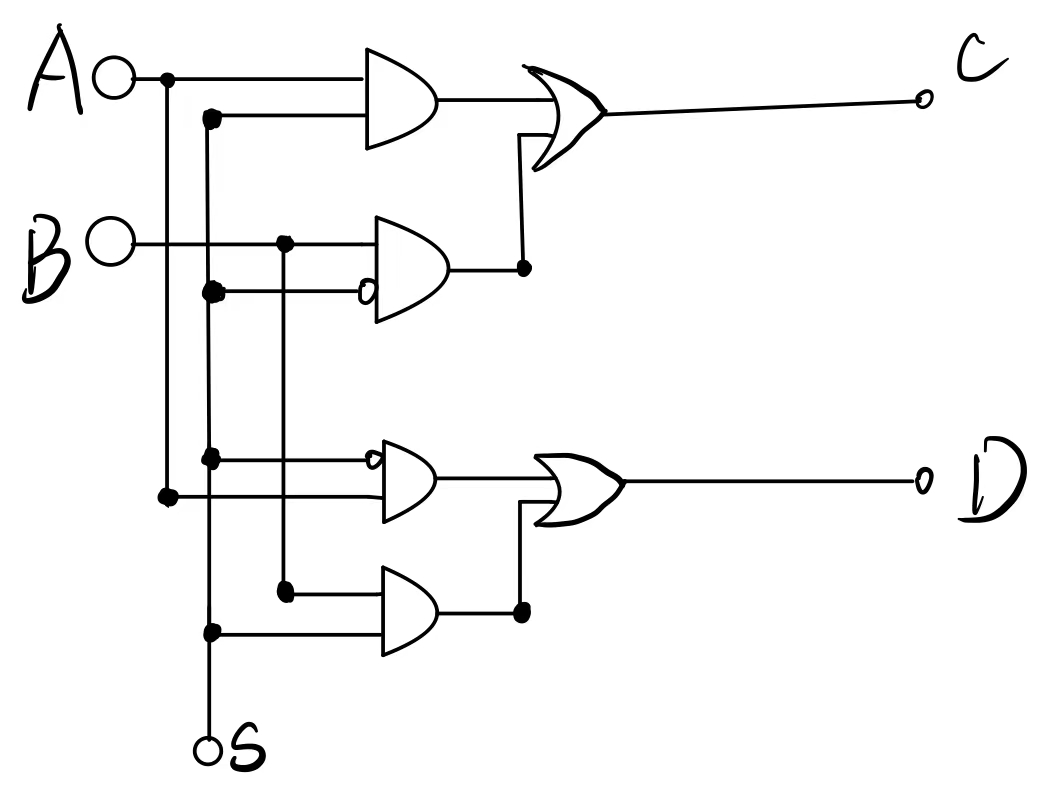
\includegraphics{answerB14.png}

\problem{B.24}(6 points) The ALU supported set on less than (\texttt{slt}) using just the sign bit of the adder.  Let's try a set on less than operation using the values $-7_\text{ten}$ and $6_\text{ten}$.  To make it simpler to follow the example, let's limit the binary representations to 4 bits $1001_\text{two}$ and $0110_\text{two}$.
\[ 1001_\text{two} - 0110_\text{two} = 1001_\text{two} + 1010_\text{two} = 0011_\text{two} \]
This result would suggest that $-7 > 6$, which is clearly wrong.  Hence, we must factor in overflow in the decision.  Modify the 1-bit ALU in Figure B.5.10 on page B-33 to handle \texttt{slt} correctly.  Make your changes on a photocopy of this figure to save time. (Section B.5)

\answer
You may draw this solution and upload an image, or include it here:
%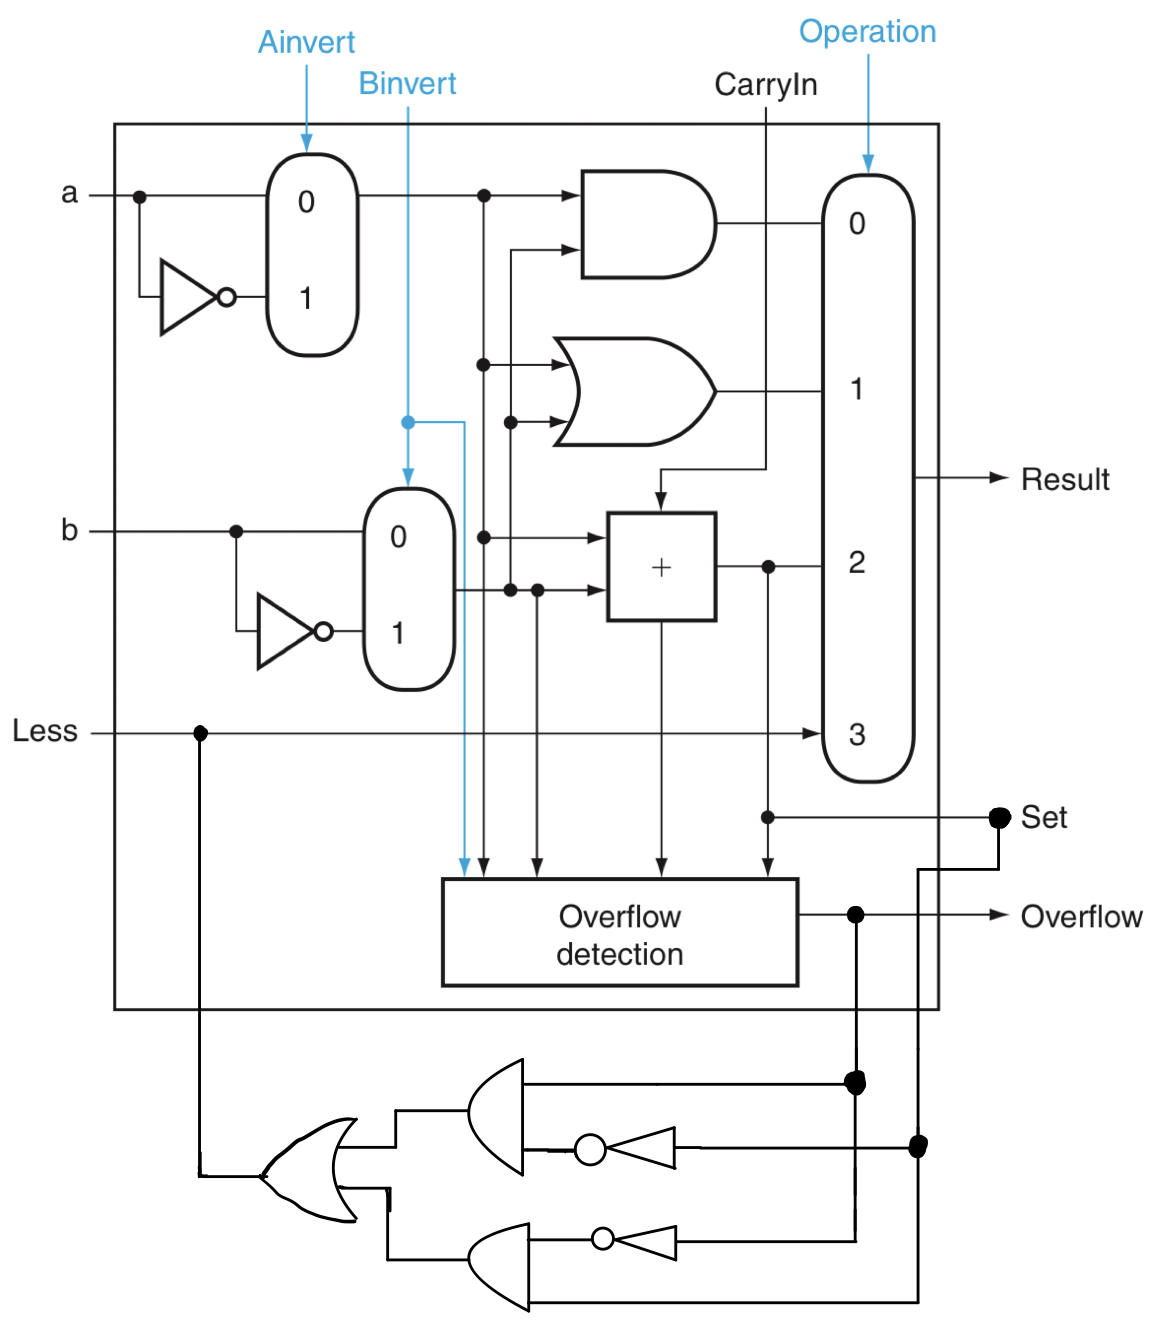
\includegraphics{answerB24.png}

\problem{B.36}(10 points) Figure~B.8.8 on page~B-55 illustrates the implementation of the register file for the MIPS datapath.  Pretend that a new register file is to be built, but that there are only two registers and only one read port, and that each register has only 2 bits of data.  Redraw Figure~B.8.8 so that every wire in your diagram corresponds to only 1 bit of data (unlike the diagram in figure~B.8.8, in which some wires are 5 bits and some wires are 32 bits).  Redraw the registers using D flip-flops.  You do not need to show how to implement a D flip-flop or a multiplexor. (Section B.8)

\answer
You may draw this solution and upload an image, or include it here:
%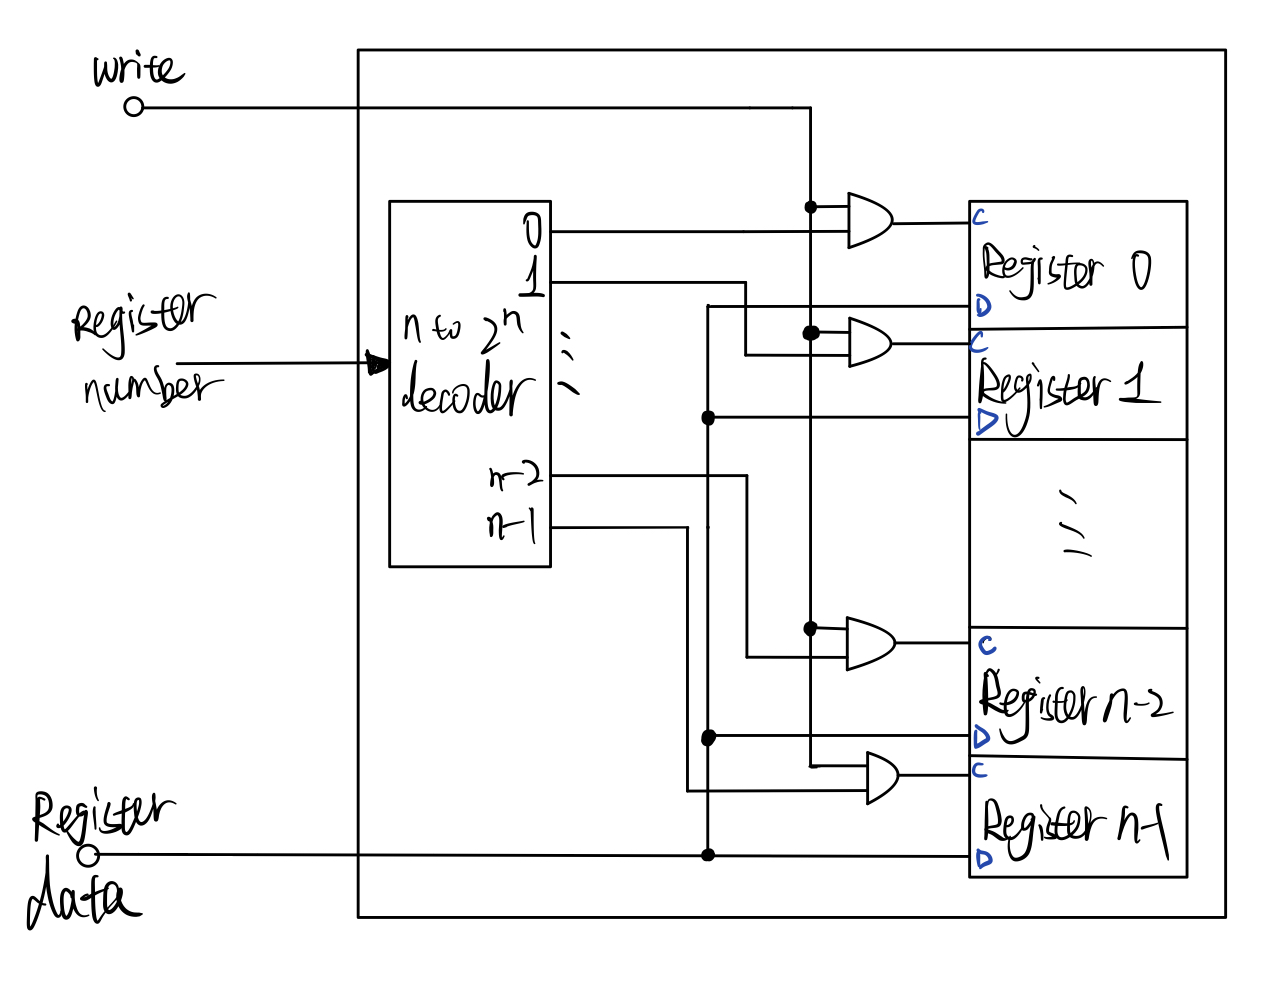
\includegraphics{answerB36.png}

\end{document}
